%
% File acl2019.tex
%
%% Based on the style files for ACL 2018, NAACL 2018/19, which were
%% Based on the style files for ACL-2015, with some improvements
%%  taken from the NAACL-2016 style
%% Based on the style files for ACL-2014, which were, in turn,
%% based on ACL-2013, ACL-2012, ACL-2011, ACL-2010, ACL-IJCNLP-2009,
%% EACL-2009, IJCNLP-2008...
%% Based on the style files for EACL 2006 by 
%%e.agirre@ehu.es or Sergi.Balari@uab.es
%% and that of ACL 08 by Joakim Nivre and Noah Smith

\documentclass[11pt,a4paper]{article}
\usepackage[hyperref]{acl2019}
\usepackage{times}
\usepackage{latexsym}
\usepackage[utf8]{inputenc}
\usepackage[T2A,T1]{fontenc}
\usepackage[ukrainian,english]{babel}
\usepackage{graphicx}


\usepackage{url}

%\aclfinalcopy % Uncomment this line for the final submission
%\def\aclpaperid{***} %  Enter the acl Paper ID here

%\setlength\titlebox{5cm}
% You can expand the titlebox if you need extra space
% to show all the authors. Please do not make the titlebox
% smaller than 5cm (the original size); we will check this
% in the camera-ready version and ask you to change it back.

\newcommand\BibTeX{B\textsc{ib}\TeX}

\title{Unsupervised induction of Ukrainian morphological paradigms for the new lexicon: extending coverage for Named Entities and neologisms using inflection tables and unannotated corpora.}
%\title{Instructions for ACL 2019 Proceedings}


\author{First Author \\
  Affiliation / Address line 1 \\
  Affiliation / Address line 2 \\
  Affiliation / Address line 3 \\
  \texttt{email@domain} \\\And
  Second Author \\
  Affiliation / Address line 1 \\
  Affiliation / Address line 2 \\
  Affiliation / Address line 3 \\
  \texttt{email@domain} \\}

\date{}

\begin{document}
\maketitle
\begin{abstract}
	The paper presents an unsupervised method for quickly extending a Ukrainian lexicon by generating paradigms and morphological feature structures for new Named Entities and neologisms, which are not covered by existing static morphological resources. This approach addresses a practical problem of modelling paradigms for entities created by the dynamic processes in the lexicon: this problem is especially serious for highly-inflected languages in  domains with specialised or quickly changing lexicon. The method uses an unannotated Ukrainian corpus and a small fixed set of inflection tables, which can be found in traditional grammar textbooks. The advantage of the proposed approach is that updating the morphological lexicon does not require training or linguistic annotation, allowing fast knowledge-light extension of an existing static lexicon to improve morphological coverage on a specific corpus. The method is implemented in an open-source package on a GitHub repository \url{https://github.com/qumtie/paralex4morphosyntax}. It can be applied to other low-resourced inflectional languages which have internet corpora and linguistic descriptions of their inflection system, following the example of inflection tables for Ukrainian. Evaluation results shows consistent improvements in coverage for Ukrainian corpora of different corpus types.
	

\end{abstract}

%\begin{abstract}
%  This document contains the instructions for preparing a camera-ready
%  manuscript for the proceedings of ACL 2019. The document itself
%  conforms to its own specifications, and is therefore an example of
%  what your manuscript should look like. These instructions should be
%  used for both papers submitted for review and for final versions of
%  accepted papers.  Authors are asked to conform to all the directions
%  reported in this document.
%\end{abstract}

\section{Introduction}


\begin{quote}
	"Our language can be regarded as an ancient city: a maze of little streets and squares, of old and new houses, of houses with extensions from various periods, and all this surrounded by a multitude of new suburbs with straight and regular streets and uniform houses." \cite{Wittgenstein-2009}
\end{quote}
This metaphor from Wittgenstein's later work `Philosophical Investigations' may be applied to two aspects of the natural language lexicon, which so far have received little attention in computational linguistics. Firstly, like a city, the lexicon constantly evolves, reflecting political and technical changes in the society that take place very rapidly, so it may be insufficient to design static lexical resources and to expect that they would give the same high level of corpus coverage once and for all: the lexicon needs to be constantly updated to reflect live changes in the system. Secondly, even though there may be many irregularities in the lexicon, similar to `a maze of little streets', this more often happens with an older lexical core, while new words typically follow more `straight and regular' patterns, so the task of updating the lexicon for natural language applications may be facilitated by this tendency.

This paper investigates the extent of the new lexicon problem for different types of Ukrainian corpora and further proposes and evaluates a knowledge-light approach to extending lexical coverage of morphological resources to neologisms (new words, meanings or usages) and new Named Entities which follow regular inflectional patterns.

Morphological annotation of the lexicon is an important component for many natural language processing pipelines, such as part-of-speech tagging, morphological disambiguation, parsing, semantic analysis, as well as for applications such as machine translation, information extraction, terminology detection, etc. For example, in part-of-speech tagging the morphological lexicon normally supplies lemmas and associated sets of possible parts-of-speech and values of morphological categories for each token (e.g., for Ukrainian this would be values for the grammatical case: nominative, genitive, dative, accusative, instrumental, locative, vocative; number: singular, plural; gender: masculine, feminine, neuter; person: 1st, 2nd, 3rd; mood: indicative, imperative, subjunctive; tense: past, present, future, etc.). The tagger then resolves any potential ambiguity using transition probabilities, trained neural networks, etc. For any language the creation of a morphological lexicon is difficult, because of a large number of lexical types needed to achieve good corpus coverage and also because of irregularities in word paradigms (systems of inflected word forms, lemmas and associated morphological features). For highly inflected Slavonic languages the creation of the morphological lexicon is even more challenging, since most words have complex morphological paradigms, which require fine-grained annotation of parts-of-speech and their grammatical sub-categories. Creation of high-quality morphological resources for these languages often requires an extensive effort over many years.

Like the majority of other Slavonic languages, Ukrainian is a highly inflected language with the `synthetic' grammar structure (where grammatical relations are predominantly marked within content word forms), so the task of morphological paradigm generation for it is not trivial. It is also more critical for the accuracy of related tasks, such as part-of-speech tagging, because of a larger potential number of combinations of possible morphological values: it is harder to guess the correct part-of-speech tag based on neighbouring tags in the case of a missing word form. Ukrainian paradigms for inflected parts of speech have between 7 and 28 distinct morphological feature combinations and associated word forms for a single lemma, and there is both regular and irregular ambiguity within and across different parts-of-speech and lexicogrammatical classes of words (i.e., animate vs. inanimate nouns, perfective vs. imperfective verbs). In Ukrainian, as in other highly-inflected languages most morphological information is supplied within the word rather than by the context, so lexical gaps are more detrimental for correct prediction of inflected word forms and their morphological characteristics.

For Ukrainian there exist wide-coverage lexical resources (see Section~\ref{sec:PrevWork}), however, extending them in a traditional rule-based way would involve continuous annotation effort requiring linguistic expertise and near-native knowledge of the language, making it hard to keep up with most recent lexical developments. 

The approach proposed in this paper is designed for the scenario where for a highly-inflected language there exists a hand-crafted static morphological lexicon that covers potentially irregular and more frequent lexical core. For extending this lexicon to cover new regularly inflected entities we use an internet corpus and small inflection tables from grammar textbooks, e.g., \cite{hryshchenko1997sulm}, \cite{press2015ukrainian}: such resources would often be available for other low-resourced languages, since the tasks that would require linguistic expertise (i.e., creating the core lexicon and inflection tables) need to be done only once, so paradigms for new entities can be automatically created whenever a new corpus becomes available. Core static morphological lexicons have been developed for several low-resourced languages, either as stand-alone resources or within shared frameworks, such as Universal Dependencies \cite{nivre2016universal}, Apertium \cite{forcada2011apertium} (in the context of Machine Translation) or Grammatical Framework \cite{ranta11gram} (in limited subject domains). However, the task of extending morphological lexicon in response to dynamic processes in the lexical system, emergence of neologisms, new terminology or Named Entities has not been systematically addressed so far.

The paper is organised as follows. In Section~\ref{sec:PrevWork} we review some of the previous work in the area, in Section~\ref{sec:Algorithm} we describe the algorithm, datasets and an experiment on generating paradigms, in Section~\ref{sec:Evaluation} we present experimental results on comparative evaluation of lexical coverage on different corpora for the baseline static morphological lexicon and for the extended paradigms which cover the new lexicon. Section~\ref{sec:Discussion} presents a discussion of examples of identified new entities and in Section~\ref{sec:Conclusions} we summarise conclusion and ideas for future work.

\section{Previous work}
\label{sec:PrevWork}

Several projects have addressed the problem of developing the Ukrainian morphological lexicon and morphological disambiguation strategies:~\cite{gryaznukhina-ed-1989}, \cite{gryaznukhina-ed-1999}, \cite{Rysin-Starko-2019}, \cite{kotsyba2009ugtag}, \cite{kotsyba2010multext}, \cite{babych2016ukrainian}. For the experiments presented in this paper we use the most complete morphological toolkit from \cite{Rysin-Starko-2019}, which in its current implementation contains a wide-coverage lexicon: 366,846 Ukrainian lemmas, which are expanded into 5,690,688 word forms with corresponding morphological feature combinations.

We evaluate the coverage of this lexicon on large Ukrainian corpora collected in lang-uk project \cite{Dyomkin-2019}, Table~\ref{lang-uk-corpus-description} is taken from this source, which describes these collections.


\begin{table}[]
	\begin{center}
		\begin{tabular}{|l|rr|}
			\hline \textbf{Corpus} & \textbf{No of words} & \textbf{No of sent} \\ \hline
			News & 461,451,019 & 31,021,650 \\
			Wikipedia & 185,645,357 & 15,786,948 \\
			Fiction & 18,323,509 & 1,811,548 \\
			Law  & 578,988,264 & 29,208,302 \\
			\hline
			Total & 1,244,408,149 &  77,828,448\\
			\hline
		\end{tabular}
	\end{center}
	\caption{\label{lang-uk-corpus-description} Description of Ukrainian corpora from \cite{Dyomkin-2019}. }
\end{table}


Detailed overviews of different approaches to developing morphological lexicons can be found in \cite{ahlberg2015paradigm}, \cite{koskenniemi2018guessing} and  \cite{fam2018ips}. For our purposes the existing approaches can be characterised by their application scenarios and assumptions about available datasets. Interesting work has been done within the neural, supervised and semi-supervised frameworks, e.g., \cite{ahlberg2015paradigm}, \cite{hulden2014semi}, \cite{koskenniemi2018guessing}, \cite{silfverberg2018computational}, \cite{wolf2018structured}, \cite{kirov2018recurrent}, \cite{faruqui2016morpho}, \cite{faruqui2015morphological}, \cite{aharoni2016morphological}, \cite{cotterell2017paradigm}. Much of this work assumes availability of partially labeled data, such as word paradigms and/or clean datasets, such as lists of `headwords' (lemmas) from which paradigms are generated. \cite{fam2018ips} identify three main approaches to learning morphological inflection: the hand-engineered rule-based approach, which requires much cost and time for construction, the supervised approach, which relies on initial labelled datasets and the neural approach, which needs more training time and even more data. However, for low-resource scenarios more attention need to be given to unsupervised knowledge-light methods, which could make strong assumptions, e.g., based on compact  linguistic descriptions of the inflection systems, but for the most part rely only unlabelled data or resources that would be typically available for low-resource languages.

A terminological note: in several papers, such as \cite{ahlberg2015paradigm}, \cite{silfverberg2018computational}, the term `paradigm' is used to describe a generalised inflection pattern, which could apply to a class of words, while the term `inflection table' characterises an individual system of inflection for a single word. This usage differs from the traditional understanding of the notion of a paradigm as a system of word forms for a given word, see e.g., \cite{spencer2001paradigm}. In our paper we adhere to the traditional terminological usage for the term `paradigm' as a system of word forms, and use the term `inflection tables' referring only to tables of inflections, which may be attached to a class of stems.

The problem of characterising dynamic processes in the Ukrainian lexicon has been discussed in \cite{klymenko2008dynamichni}, \cite{karpilovska2013aktyvni}, where these changes are attributed to political, cultural and technical developments in the society -- the active `social dynamics', which causes the active `linguistic dynamics': renewal and additions to nominative and communicative resources of the language and changes in linguistic norms. While the grammar or phonology remain more conservative, the lexicon is very open to such changes. There is an ongoing work to record these lexical developments for Ukrainian and other languages, however, so far there is no systematic computational linguistic framework for modelling morphological features and inflections for neologisms and new Named Entities.

\section{Algorithm description}
\label{sec:Algorithm}

The proposed algorithm uses small set of inflection tables for inflected parts-of-speech which accepts new entities (i.e., nouns, adjectives and verbs, but not numerals or pronouns, which are closed class entities) and unannotated corpus (or a frequency list compiled from such a corpus). It attempts to split each token in the corpus into its stem and inflection using all inflections in all available inflection tables. When a split is successful, it generates a full hypothetical paradigm consistent with the split, using the identified stem and all other inflections for the given table. Then these hypotheses are checked against available word forms in the corpus: whether a sufficient number of forms can be found to confirm the hypothetical paradigm. In this approach for the paradigms to be generated reliably, the new entities need to have a sufficient morphological diversity in the corpus: we experimentally established that at least 3 or 4 different word forms are needed to make a reasonably accurate prediction of a paradigm and its remaining unseen word forms. For confirmed paradigms the algorithm generates all remaining word forms, their lemma (as a designated `dictionary' word form in the paradigm, e.g., the nominative singular form for nouns) and their sets of morphological category values associated with inflections, based on the expected structure of the paradigm. Multiple splits of a token are possible, so hypothetical paradigms are ranked by the number of confirmed word forms, and the paradigm with the highest number is selected among the competing paradigms. Figure \ref{fig:alg1} shows the general overview of the algorithm.

\begin{figure}
	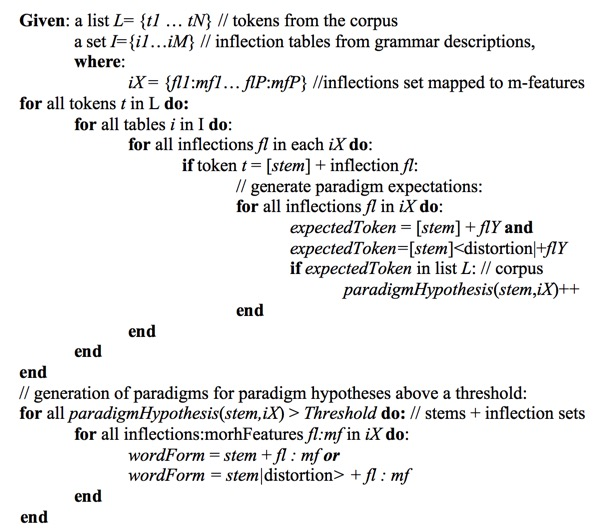
\includegraphics[width=\linewidth]{algorithm-description.jpg}
	\caption{Algorithm description.}
	\label{fig:alg1}
\end{figure}

For a general case to cover less regular paradigms with stem alternations the algorithm may be complemented with a distortion model which modifies tested tokens and hypothetical word forms according to morphonological rules of the language, for Ukrainian this would cover historical alternations such as [o,e] -> [i] in `newly closed' syllables, e.g., [kon'a] (horse.Gen.sing) -> [kin'] (horse.Nom.sing), [h, k, x] before [i] -> [z, ts, s], e.g., [ruka] (hand.Nom.sing) -> [rutsi] (hand.Dat.sing), etc.  

The example in Figure~\ref{fig:alg_example} illustrates working of the algorithm. In this example we assume that the current token is \selectlanguage{ukrainian}рука \selectlanguage{english}(ruka = `hand'), for which the algorithm will try to generate paradigms. In our dataset we have inflection tables for the `hard', `soft', `iotated' and `mixed' groups of the 1st declination of nouns, taken from a Ukrainian grammar textbook \cite{hryshchenko1997sulm}: \selectlanguage{ukrainian}фабрика, робітниця, надія, площа \selectlanguage{english}(fabryka = `factory', robitnyts'a = `worker', nadija = `hope', ploshcha = `town square'): we use only inflection sets and morphological values from these tables (the stems in the inflection tables are only for illustration).

\begin{figure*}
	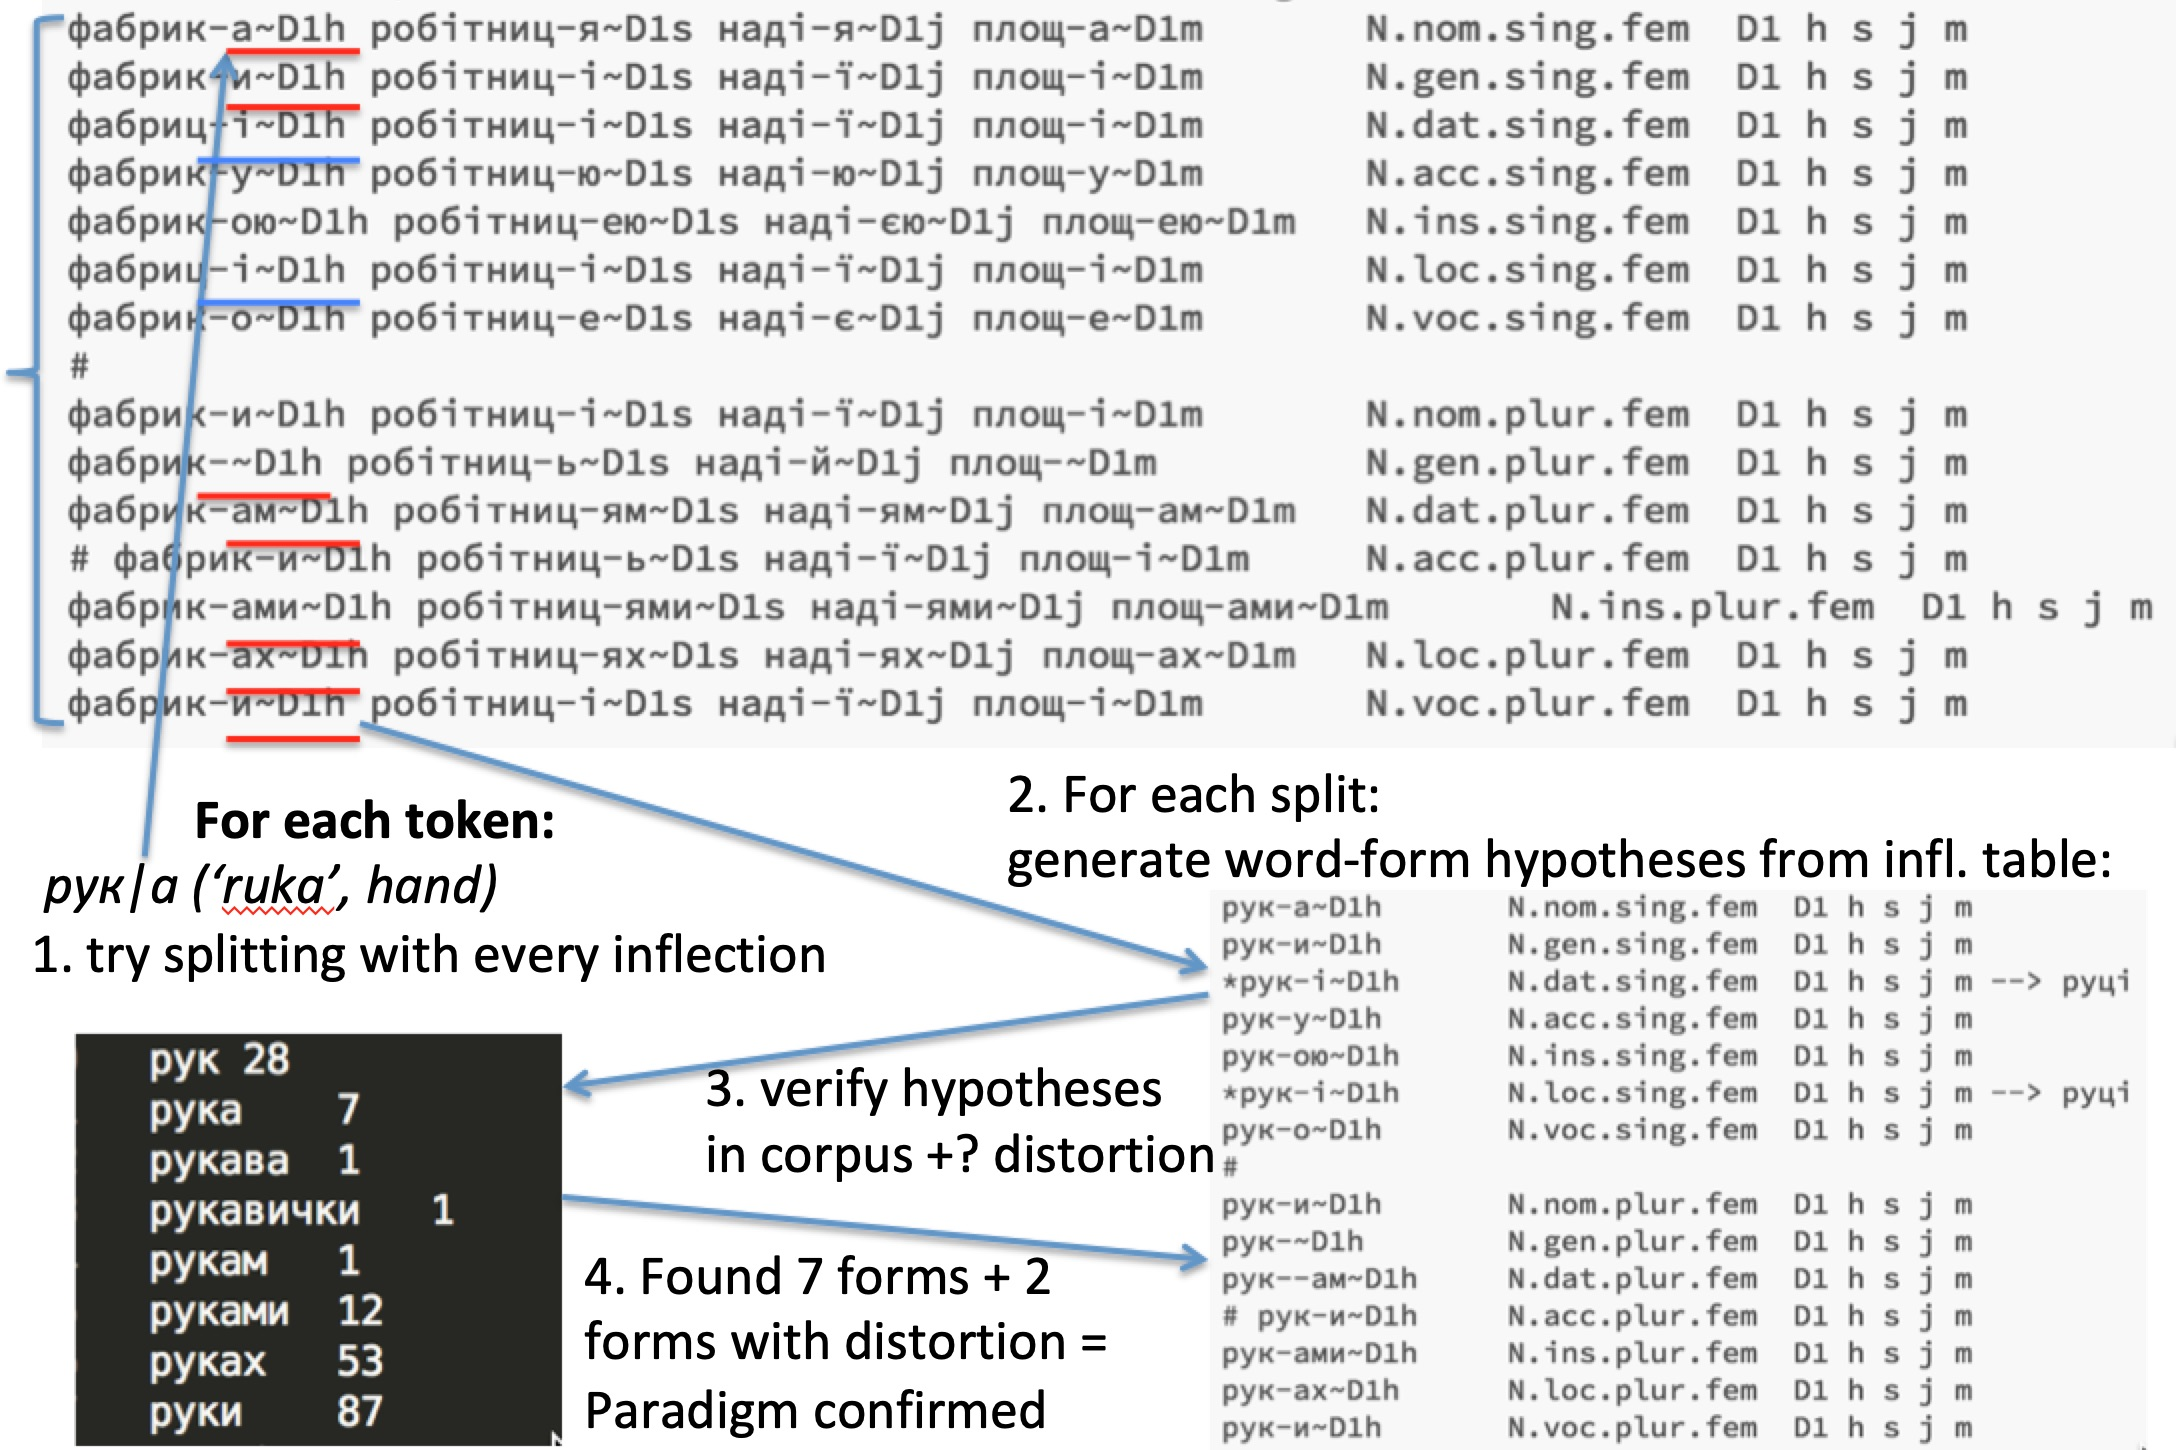
\includegraphics[width=\linewidth]{algorithm-illustration.jpg}
	\caption{Illustration of the algorithm.}
	\label{fig:alg_example}
\end{figure*}

In the first stage the algorithm tries every inflection in every table to split the current token ('ruka'). A possible split is found in the inflection table for the 1st declination of nouns, for the `hard' and `mixed' groups illustrated by examples `fabryka' and `ploshcha'. The split separates the stem \emph{'ruk'} and the inflection \emph{'a'}.

In the second stage, trying the split for the `hard' group, the word form hypotheses are generated from the inflection table: \emph{ruk+y, ruk+u, ruk+oju, ruk-o, ruk, ruk+amy, ruk+ax} and with the distortion model: [k] /\_[i] -> [ts] -- \emph{ruts+i}. For the split defined by the `mixed' group inflection table, in addition two incorrect word forms will be generated \emph{*ruk+eju, *ruk-e}, but the following three correct forms will not be generated: \emph{ruk-y, ruk-oju, ruk-o}. Therefore, two paradigms for the split \emph{ruk|a} will be competing with each other.

In the third stage, each of the competing paradigms will be verified against the corpus: in our example, for the `hard' group the following four hypothesised word forms are actually found: \emph{ruk, ruk+am, ruk+ax, ruk+y}, which, together with the 5th original form \emph{ruk+a}, correspond to 7 morphological feature combinations, since \emph{ruk+y} is ambiguous having three interpretations. While for the `mixed' group only three hypothesised forms will be confirmed + initial \emph{ruk+a} = 4, because the existing form \emph{ruk+y} has not been predicted by the `mixed' paradigm. As a result, the correct `hard' paradigm will be ranked higher, with 5 confirmed word form hypotheses vs. 4 confirmed hypotheses for the wrong `mixed' paradigm. When the corpus gets larger, more clues may differentiate such closely competing paradigms and more correct rankings may be produced.

In the fourth stage the top-ranking paradigm is confirmed and previously unseen word forms are generated, as well as possible part-of-speech code, lemma and all possible morphological feature combinations for both seen and unseen word forms, such as values for case, number, gender, e.g., the unseen word form \emph{ruk+u} will be generated with its morphological information \emph{ruk-u : lem=ruka; PoS=N.acc.sing}, etc.

Note that for a single token it is not possible to clearly distinguish between a competing wrong paradigm and an alternative legitimate paradigm, which corresponds to a different reading of an ambiguous word form. For example, the word form \emph{pryklad|y} belongs both to \emph{PoS=N.nom.plur; lemma=pryklad (`example')} and to \emph{PoS=V.imper.pers2.sing; lemma=pryklasty/pryklad+u (`to attach')}. The limitation of the algorithm is that only one of these correct paradigms is confirmed for the given word form \emph{pryklady}, depending on how many hypothesised word forms are found in corpus for each of the verbal or nominal paradigms. However, the same paradigm is confirmed via different routes, i.e., through splitting other word forms belonging to the same paradigm, e.g., in Figure~\ref{fig:alg_example} the paradigm for \emph{lemma=ruka, PoS=N} will be also confirmed via splitting the corpus tokens \emph{ruk|am, ruk|amy, ruk|ax}. This gives the proposed algorithm an advantage, compared to the approach described in \cite{ahlberg2015paradigm} for the case of overlapping paradigms with ambiguous word forms: alternative readings will be confirmed by the tokens in corpus which are unique for each of the alternative paradigms, e.g., \emph{pryklad+ut' (`they will attach')} vs. \emph{pryklad+om (`with an example')}. Interestingly, ambiguous word forms are not discarded: when unambiguous tokens are split for each of the overlapping paradigms, the ambiguous tokens will count in both cases to confirm both of the correct paradigms. This will not happen for competing wrong paradigms: their wrong word form predictions (such as \emph{*ruk+eju} in the example above)  will simply not be found in corpus, so they will not initiate the process for the alternative paradigm.

For the purposes of this experiment we evaluate the coverage given by the algorithm without a distortion model, as such alternations are more typical for the older lexicon and often do not occur in recently borrowed items, e.g. [portu] (port.Gen.sing) - port (port.Nom.sing): [o] -> [i] alternation does not take place, as the word was borrowed after the phonological law of the `open syllable' no longer worked in Ukrainian. However, in future the distortion models may be learnt from data or directly coded as explicit linguistic knowledge, and in this way the older paradigms and live stem alternations may also be covered.



\section{Evaluating algorithm with corpus coverage}
\label{sec:Evaluation}

The algorithm is used for extending the Ukrainian morphological lexicon from four corpora: news, wikipedia, law and fiction, and from a combined corpus that merges these four corpora. Table~\ref{lang-uk-corpus-generation} shows the number of word forms generated from each of the corpora presented in Table~\ref{lang-uk-corpus-description}.

\begin{table}[]
	\begin{center}
		\begin{tabular}{|l|rr|}
			\hline \textbf{Corpus} & \textbf{No of generated word forms} & \textbf{ } 
			\\ \hline
			dict\_uk & 5,690,688  &  \\
			\hline
			News & 3,292,591 &  \\
			Wikipedia & 3,765,774 &  \\
			Fiction & 958,233 &  \\
			Law & 1,788,288 &  \\
			\hline
			All corpora & 6,626,004 &  \\
			\hline
		\end{tabular}
	\end{center}
	\caption{\label{lang-uk-corpus-generation} Size of lexicon generated from corpora. }
\end{table}

We measure the coverage (in terms of lexical types) in four corpora and in the merged corpus, with gradually filtering out lower frequency ranges. The rationale for this evaluation method is that it is usually harder for the lexicon to cover low-frequent items, so we test our lexicons on a range of tasks of varying difficulty.

As the baseline, Figure~\ref{fig:pcNoTypDictUK} shows the coverage of the existing static lexicon from the dict\_uk project developed by \cite{Rysin-Starko-2019} (also characterised in the first row in Table~\ref{lang-uk-corpus-generation}). The horizontal axis indicates which frequency range has been filtered out. (Note the change of scale in the middle of the graph from 1 to 10 in one unit of length).

\begin{figure}
	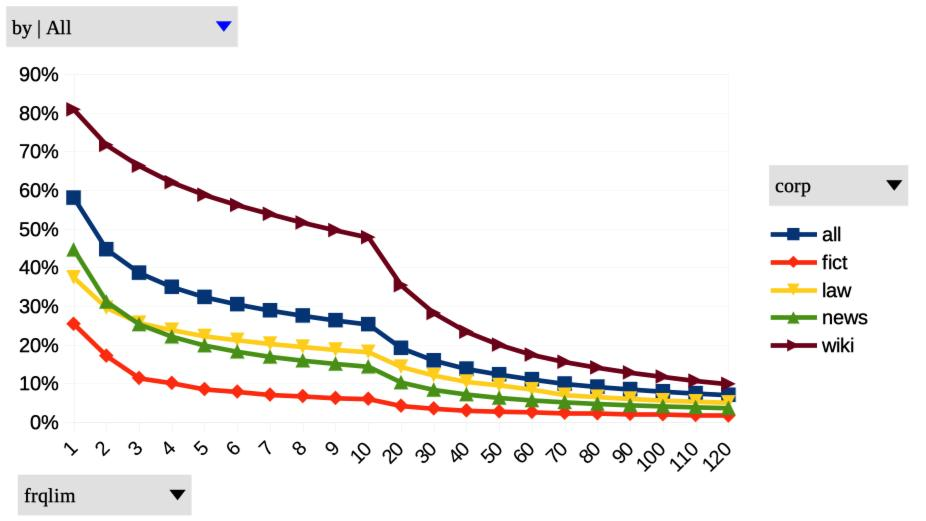
\includegraphics[width=\linewidth]{evaluation-coverage-dict_uk.jpg}
	\caption{The baseline: Percent of non-covered types (y) in dict\_uk lexicon, with filtered out lower frequencies, up to (x).}
	\label{fig:pcNoTypDictUK}
\end{figure}

It can be seen from the figure that the Wikipedia corpus that contains many Named Entities and specialised terminology is the most problematic in terms of coverage: up to 80\% of its types are not covered, which goes down only to around 50\% if the frequency threshold is reduced to 10. At the same time a `static' corpus of fiction texts is covered the best by the existing morphological lexicon.

We evaluate the effect of the proposed algorithm via measuring improvements in coverage of lexical types across the frequency ranges for filtered out items. We use different corpora for the development and evaluation, so the following figures show the corpus coverage for these different combinations (lower lines indicate better results). Figure~\ref{fig:pcNoTypWikiN} and Figure~\ref{fig:pcNoTypWikiL} show coverage levels for the Wiki corpus with paradigms generated from the News and Law corpora respectively. Figure~\ref{fig:pcNoTypNewsW} and Figure~\ref{fig:pcNoTypNewsL} show coverage for the News corpus with paradigms developed from the Wiki and Law corpora. Finally, Figure~\ref{fig:pcNoTypLawW} and Figure~\ref{fig:pcNoTypLawN} show coverage for the Law corpus with paradigms developed from the Wiki and News corpora. In these figures the baseline graphs labelled `wiki', `news' and `law' are the same as shown in Figure~\ref{fig:pcNoTypDictUK}.

\begin{figure}
	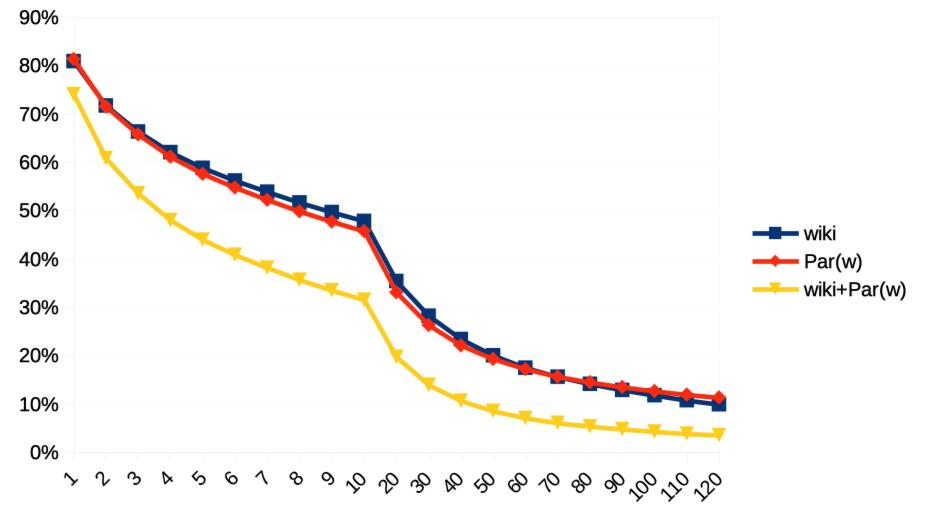
\includegraphics[width=\linewidth]{evaluation-coverage-wikiN.jpg}
	\caption{Percent of non-covered types (y) in Wiki corpus, with dict\_uk (`wiki' line), with only our algorithm and paradigms generated from News corpus (`Par(w)' line), and with the two morphological lexicons combined (wiki+Par(w) line); filtered out lower frequencies, up to (x).}
	\label{fig:pcNoTypWikiN}
\end{figure}

\begin{figure}
	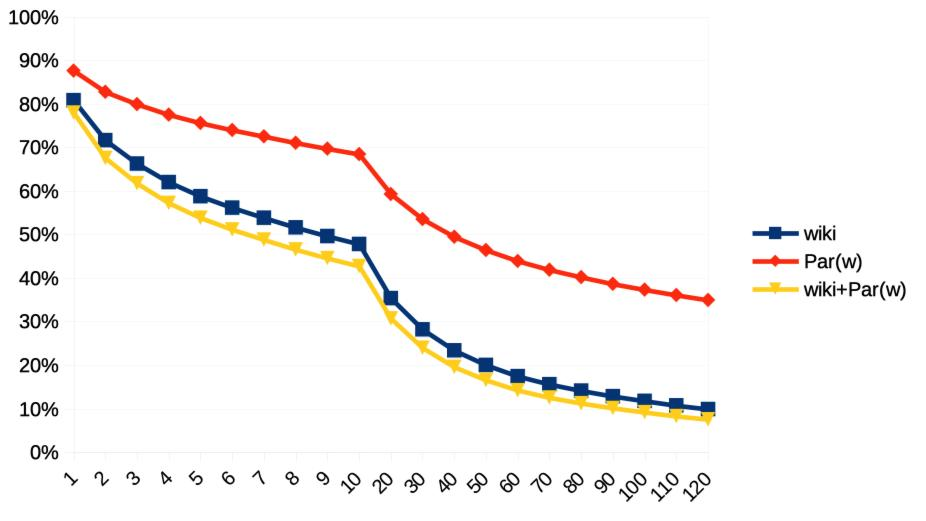
\includegraphics[width=\linewidth]{evaluation-coverage-wikiL.jpg}
	\caption{Percent of non-covered types (y) in Wiki corpus, with dict\_uk (`wiki' line), with only our algorithm and paradigms generated from Law corpus (`Par(w)' line), and with the two morphological lexicons combined (wiki+Par(w) line); filtered out lower frequencies, up to (x).}
	\label{fig:pcNoTypWikiL}
\end{figure}


\begin{figure}
	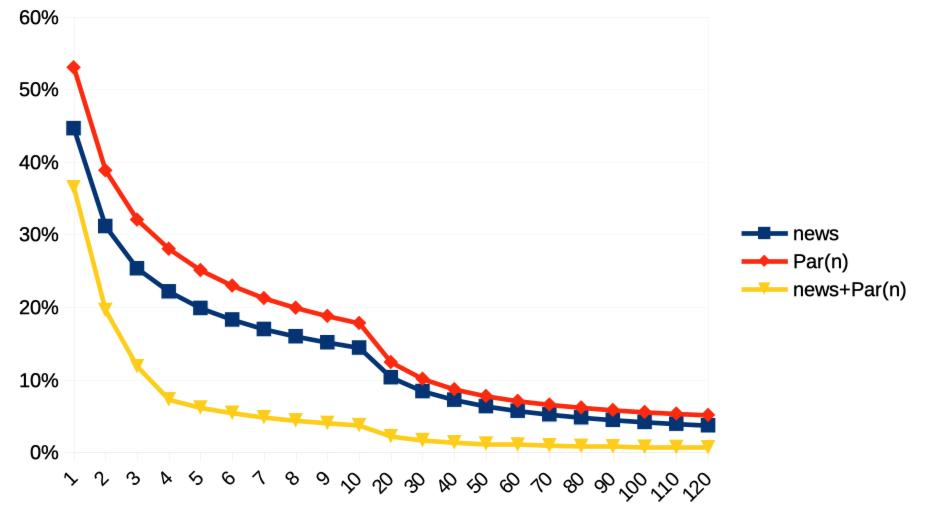
\includegraphics[width=\linewidth]{evaluation-coverage-newsW.jpg}
	\caption{Percent of non-covered types (y) in News corpus, with dict\_uk (`news' line), with only our algorithm and paradigms generated from Wiki corpus (`Par(n)' line), and with the two morphological lexicons combined (news+Par(n) line); filtered out lower frequencies, up to (x).}
	\label{fig:pcNoTypNewsW}
\end{figure}

\begin{figure}
	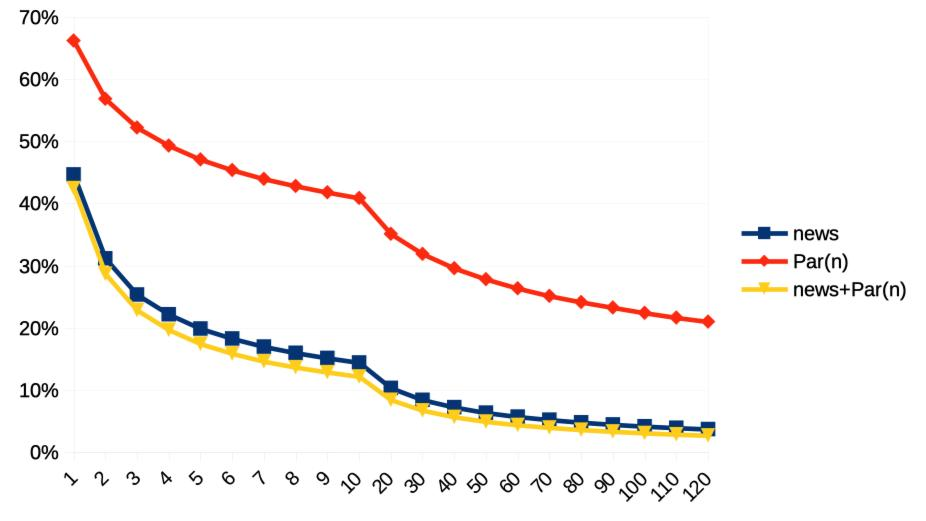
\includegraphics[width=\linewidth]{evaluation-coverage-newsL.jpg}
	\caption{Percent of non-covered types (y) in News corpus, with dict\_uk (`news' line), with only our algorithm and paradigms generated from Law corpus (`Par(n)' line), and with the two morphological lexicons combined (news+Par(n) line); filtered out lower frequencies, up to (x).}
	\label{fig:pcNoTypNewsL}
\end{figure}


\begin{figure}
	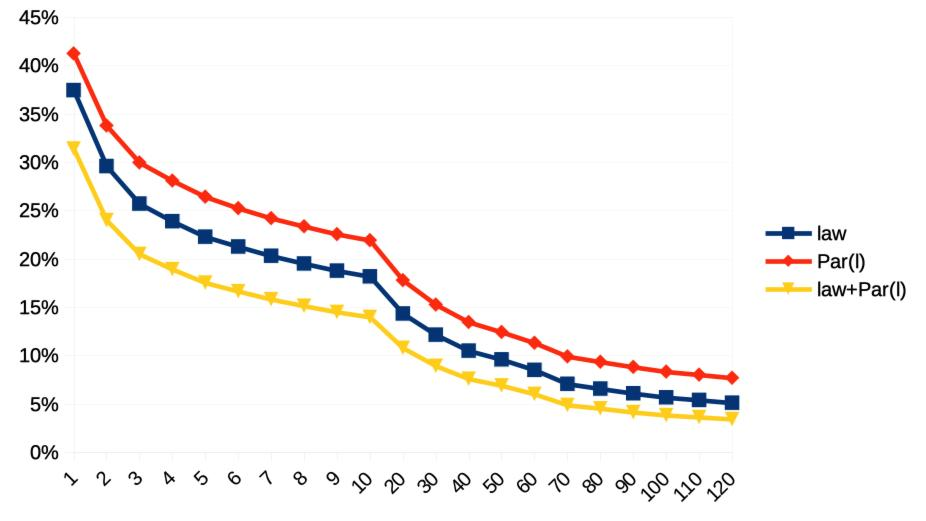
\includegraphics[width=\linewidth]{evaluation-coverage-lawW.jpg}
	\caption{Percent of non-covered types (y) in Law corpus, with dict\_uk (`law' line), with only our algorithm and paradigms generated from Wiki corpus (`Par(l)' line), and with the two morphological lexicons combined (law+Par(l) line); filtered out lower frequencies, up to (x).}
	\label{fig:pcNoTypLawW}
\end{figure}

\begin{figure}
	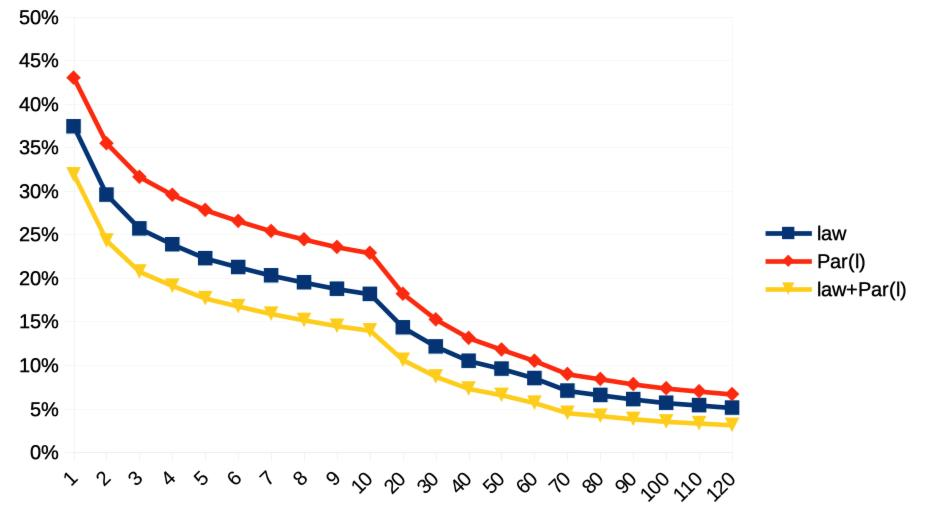
\includegraphics[width=\linewidth]{evaluation-coverage-lawN.jpg}
	\caption{Percent of non-covered types (y) in Law corpus, with dict\_uk (`law' line), with only our algorithm and paradigms generated from News corpus (`Par(l)' line), and with the two morphological lexicons combined (law+Par(l) line); filtered out lower frequencies, up to (x).}
	\label{fig:pcNoTypLawN}
\end{figure}


It can be seen from the figures that for our algorithm the morpholigical and lexical diversity of the corpus are essential: the Law corpus has very little effect on the coverage of both News and Wikipedia corpora, while the News and Wikipedia consistently improve the coverage of all the corpora on which they are evaluated. This may be due to the small type/token ratio (i.e., small lexical diversity) of the Law corpus.

Finally, Figures~\ref{fig:pcDiffNoTypNews} and \ref{fig:pcDiffNoTypWiki} summarise improvement rates (i.e., the difference between the baseline and the proposed approach) for all the corpora using the News and Wiki corpora for generating paradigms.

\begin{figure}
	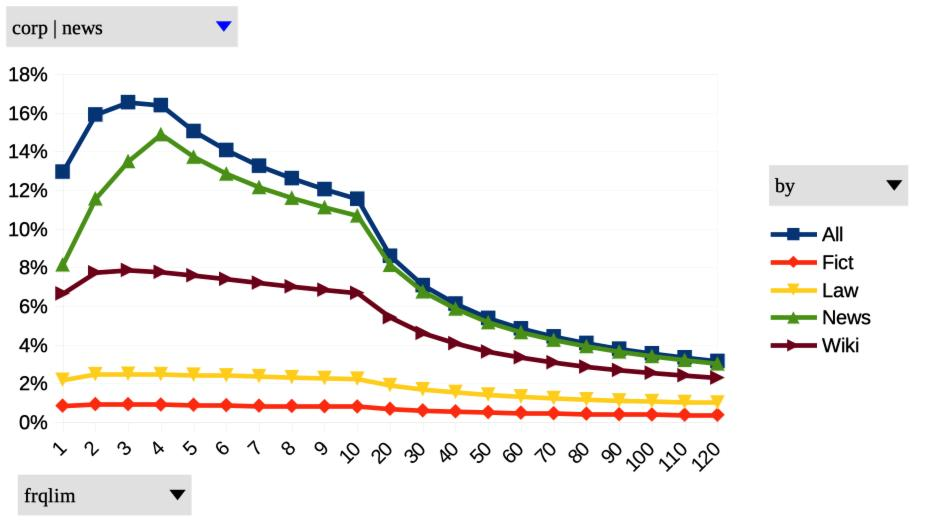
\includegraphics[width=\linewidth]{evaluation-improv-DiffNoTypNews.jpg}
	\caption{Improvement rates (y), of different corpora with the paradigms generated from New corpus; filtered out lower frequencies, up to (x).}
	\label{fig:pcDiffNoTypNews}
\end{figure}

\begin{figure}
	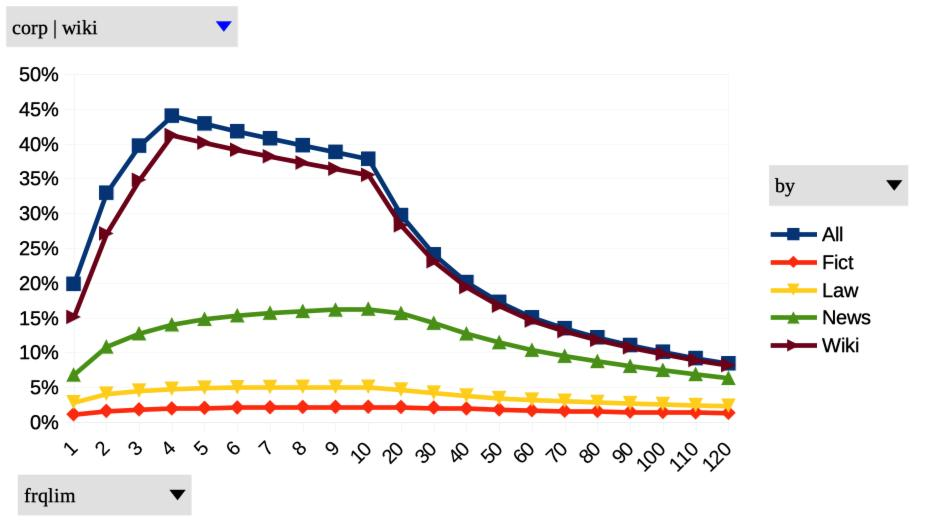
\includegraphics[width=\linewidth]{evaluation-improv-DiffNoTypWiki.jpg}
	\caption{Improvement rates (y), of different corpora with the paradigms generated from Wiki corpus; filtered out lower frequencies, up to (x).}
	\label{fig:pcDiffNoTypWiki}
\end{figure}


It can be seen from these figures that the coverage of Fiction and Law corpora is harder to improve, while News and Wiki corpora are most complementary, improving each other well. Also an interesting effect can be observed when a corpus is used to improve itself: the improvement rate peaks at the value of filtered frequencies up to 4, which may be interpreted as improvement in reliability of paradigm prediction for more frequent items, and as an indication of a possible threshold for the minimal number of slots for predicting Ukrainian paradigms.

The results indicate that the proposed approach gives consistent improvements in coverage with paradigms generated from a lexically diverse corpora with sufficient number of neologisms and new named entities. The highest improvement rates across different corpora has been achieved for paradigms generated from the Wiki corpus used to test the News corpus -- 16.3\% for lexical items with frequencies 10 and higher.


\section{Discussion}
\label{sec:Discussion}

Most lexical items covered with the proposed paradigm generation algorithm are Named Entities -- names of organisations, geographical places or people, as well as technical terms, e.g.: \selectlanguage{ukrainian}мінохоронздоров'я \selectlanguage{english} (`The Ministry of Health') 
\selectlanguage{ukrainian}інтербізнесконсалтинг \selectlanguage{english} (`Internet business consulting'), \selectlanguage{ukrainian}кременчукм'ясо \selectlanguage{english} (`The Meat of Kremenchuk' company), \selectlanguage{ukrainian}кривбасводопостачання \selectlanguage{english} (`Kryvbas Water Supply'), \selectlanguage{ukrainian}броваритепловодоенергія \selectlanguage{english} (`Brovary Heating, Water and Energy' company), \selectlanguage{ukrainian}могадішо \selectlanguage{english} (`Mogadishu')
\selectlanguage{ukrainian}озоноруйнуючих \selectlanguage{english}. (`ozone-destroying'). 

However, the list also contains interesting political lexicon, such as \selectlanguage{ukrainian}йолка \selectlanguage{english} (`Christmas tree': the distorted ukrainized spelling of the Russian word, which became a symbol of the people's resistance to political violence during the Ukrainian revolution of dignity in 2013-2014) and \selectlanguage{ukrainian}проффесор \selectlanguage{english} (again, a distorted spelling of the word `professor', which was used for mocking the fugitive pro-Russian president, who held this title, but allegedly misspelt it in an official document). 

The appearance of this politically charged lexicon is in line with Karpilovs'ka et al.'s \shortcite{karpilovska2013aktyvni} suggestion that lexical changes are driven by the social dynamics, especially at the times of major political developments. However, we also see that this political lexicon is sill much less frequent and less changeable compared to Named Entities, which dominate the new lexicon.


\section{Conclusions and future work}
\label{sec:Conclusions}


The proposed algorithm complements static linguistic resources and increases corpus coverage for new entities, such as neologisms and proper names. The highest improvements are achieved for the corpus types that typically have many neologisms, specialised terminological lexicon and Named Entities: the Wikipedia and News. These corpora are not well covered by existing morphological resources. The advantage of the proposed approach is that it uses unlabelled corpora and small inflection tables for unsupervised induction of paradigms. However, its limitation is that in this stage it doesn't predict irregular paradigms. 

Future work will involve the development of distortion models to cover less regular cases and a systematic evaluation of the accuracy of paradigm prediction for different frequency ranges: while for more frequent items such prediction is highly reliable, there is a need to experimentally establish frequency and coverage thresholds for different error rates on this task for less frequent items. Another area for future research is the use of contextual and syntactic features to verify predicted morphological properties.

The inflection tables for Ukrainian used in the experiment and the software code for generating paradigms from corpora, which implements the proposed algorithm, are released on GitHub repository: \url{https://github.com/qumtie/paralex4morphosyntax}. 

\bibliography{acl2019}
\bibliographystyle{acl_natbib}



\end{document}
